% =====================================================================
%  Operating-point optimisation for a gate-defined Majorana channel on a
%  twisted-cuprate / topological-insulator heterostructure
%
%  Compile on Overleaf with pdfLaTeX.  revtex4-2 is installed by default.
%  Figures: run  python paper/make_figures.py  first (writes paper/figs/).
% =====================================================================
\documentclass[aps,prb,twocolumn,superscriptaddress,floatfix,nofootinbib]{revtex4-2}

\usepackage{graphicx}
\usepackage{amsmath,amssymb}
\usepackage{bm}
\usepackage[colorlinks=true,linkcolor=blue,citecolor=blue,urlcolor=blue]{hyperref}
\usepackage{xcolor}

\graphicspath{{figs/}}

\newcommand{\dtop}{\Delta_{\rm top}}
\newcommand{\vz}{V_z}
\newcommand{\vzc}{V_{z,\rm crit}}
\newcommand{\kB}{k_{\rm B}}

\begin{document}

\title{Operating-point optimisation for a gate-defined Majorana channel
proximitised by a twisted cuprate bilayer}

\author{Justin Grady}
\affiliation{Variable Systems, United States}
\email{[contact]}

\date{\today}

\begin{abstract}
Proposals for Majorana zero modes in twisted-cuprate heterostructures have
focused on vortex-bound modes, where the topological gap descends from the
induced pairing through a chain of structural suppressions. We analyse instead
a Zeeman-driven, gate-defined quasi-one-dimensional channel on a
three-dimensional topological-insulator surface proximitised by a
$45^\circ$-twisted Bi$_2$Sr$_2$CaCu$_2$O$_{8+\delta}$ bilayer, and show that
its operational gap is first order in the induced pairing. Exact
diagonalisation of the Bogoliubov--de Gennes Hamiltonian gives the bound
$\dtop \le \Delta$, with equality approached at $\vz \approx 2\Delta$. The
commonly adopted choice $\vz = 1.5\Delta$ instead yields $\dtop = \Delta/2$;
re-optimising the Zeeman energy therefore very nearly doubles the operational
gap at fixed material parameters, raising the maximum operating temperature
from $0.58$~K to $1.13$~K and halving the Majorana localisation length. We map
the accessible $(\mu, \vz)$ region subject to a laboratory in-plane-field
ceiling, showing that the chemical potential is free over
$0 \le \mu \lesssim 8$~meV at a cost of $\le 8\%$ in $\dtop$, and that the
frequently quoted requirement $E_F \lesssim 8$~meV is a magnet-access
constraint rather than a materials one. Density-matrix renormalisation-group
calculations beyond mean field show the phase survives nearest-neighbour
Coulomb repulsion, and give an electrostatic disorder tolerance
$\delta\mu_{\rm rms}/\dtop \approx 0.9 \pm 0.15$. All results are conditional
on the induced pairing gap $\Delta$, which has not been measured in this
material system; we specify the single tunneling-spectroscopy experiment that
decides the architecture, show it requires only $1$~K rather than dilution
temperatures, and give the predicted spectra and decision thresholds.
\end{abstract}

\maketitle

% =====================================================================
\section{Introduction}

Topological quantum computation encodes information in the non-local fermion
parity of spatially separated Majorana zero modes (MZMs), rendering it immune
to local perturbations that do not close the protecting gap or transfer
quasiparticles across it~\cite{Kitaev2001,Nayak2008}. In the canonical
semiconductor--superconductor realisation---an InAs or InSb nanowire
proximitised by epitaxial Al~\cite{Lutchyn2010,Oreg2010}---the induced
topological gap is limited to $\dtop \sim 0.1$~meV by the Al pairing scale.
Exponential suppression of thermal quasiparticle poisoning,
$n_{\rm qp} \propto e^{-\dtop/\kB T}$, then requires
$\kB T \lesssim \dtop/20$, i.e.\ operation at the $20$~mK mixing chamber of a
dilution refrigerator.

The protection requirement scales linearly with the gap: a tenfold larger
$\dtop$ relaxes the operating temperature tenfold. This is a size, weight,
power and cost (SWaP-C) argument as much as a physics one, because dilution
refrigerators occupy cubic metres and dominate the deployment envelope of any
fielded system.

The observation of spontaneous time-reversal-symmetry breaking consistent with
chiral $d+id'$ pairing in Bi$_2$Sr$_2$CaCu$_2$O$_{8+\delta}$ (Bi-2212)
bilayers twisted near $45^\circ$~\cite{Can2021,Zhao2023} raises the
possibility of meV-scale induced gaps in an adjacent topological insulator
(TI)~\cite{FuKane2008}. Existing proposals exploit this by placing MZMs in
Abrikosov vortex cores~\cite{Margalit2022,Zhu2023}, which requires an
out-of-plane field and produces a topological gap reduced from the induced
pairing by structural factors we discuss in Sec.~\ref{sec:comparison}.

Here we analyse the alternative: a Zeeman-driven, gate-defined quasi-1D
channel on a 3D TI surface, with MZMs at the channel endpoints and braiding by
keyboard-gated T-junction networks~\cite{Karzig2017}. Our central result is
that the operational gap of this device is bounded by the induced pairing
itself, $\dtop \le \Delta$, and that the bound is nearly saturated at a
specific Zeeman energy which prior specifications of this architecture did not
adopt.

\emph{Scope.} This is a design study. No device has been fabricated and no
measurement has been performed. Every number below is conditional on an assumed
induced pairing gap $\Delta$, which is unmeasured in this material system; we
return to this in Secs.~\ref{sec:milestone} and~\ref{sec:limitations}. We make
no room-temperature claim: at $300$~K, $\kB T = 25.9$~meV, and the criterion
$\dtop/\kB T \ge 20$ would demand a pairing gap of order $1$~eV, more than an
order of magnitude beyond any known superconductor.

% =====================================================================
\section{Model}
\label{sec:model}

The quantum channel is a gate-defined quasi-1D strip on the Bi$_2$Se$_3$
surface beneath the twisted bilayer. Its low-energy physics is captured by a
discretised Bogoliubov--de Gennes (BdG) chain of $N$ sites with lattice
constant $a = 10$~nm, in the four-component Nambu\,$\otimes$\,spin basis
$\Psi_j = (c_{j\uparrow}, c_{j\downarrow}, c^\dagger_{j\uparrow},
c^\dagger_{j\downarrow})^T$:
%
\begin{align}
H &= \tfrac{1}{2}\sum_{j=1}^{N} \Psi^\dagger_j H_{\rm on} \Psi_j
   + \tfrac{1}{2}\sum_{j=1}^{N-1}\left(\Psi^\dagger_j H_{\rm hop}\Psi_{j+1}
     + {\rm H.c.}\right), \\
H_{\rm on} &= (2t-\mu)(\tau_z\otimes\sigma_0) + \Delta(\tau_x\otimes\sigma_0)
              + \vz(\tau_0\otimes\sigma_z), \\
H_{\rm hop} &= -t(\tau_z\otimes\sigma_0) - i\alpha(\tau_z\otimes\sigma_y),
\end{align}
%
with $t = \hbar^2/2m^*a^2 = 20$~meV ($m^*\approx 0.019\,m_e$), effective
spin--orbit scale $\alpha = 10$~meV, and proximity-induced pairing $\Delta$.
The chemical potential $\mu$ is measured from the band bottom, which the
$+2t$ onsite offset makes explicit. The bulk Hamiltonian is
%
\begin{align}
H(k) =\ & [2t(1-\cos ka) - \mu](\tau_z\otimes\sigma_0)
  + 2\alpha \sin(ka)\,(\tau_z\otimes\sigma_y) \nonumber\\
  & + \Delta(\tau_x\otimes\sigma_0) + \vz(\tau_0\otimes\sigma_z).
\label{eq:hk}
\end{align}
%
Particle--hole symmetry $\mathcal{P}H(k)\mathcal{P}^{-1} = -H(-k)$ with
$\mathcal{P} = (\tau_y\otimes\sigma_y)\mathcal{K}$ and $\mathcal{P}^2=+1$
holds term by term, placing the model in Altland--Zirnbauer class D with a
$\mathbb{Z}_2$ Pfaffian invariant~\cite{Kitaev2001}.

At $k=0$ the spectrum of Eq.~(\ref{eq:hk}) separates by spin sector into
$\pm\sqrt{\mu^2+\Delta^2} + s\vz$ with $s=\pm 1$, so the bulk gap closes at
%
\begin{equation}
\vzc = \sqrt{\mu^2+\Delta^2},
\label{eq:vzcrit}
\end{equation}
%
which reduces to $\vzc = \Delta$ at the $\mu=0$ sweet spot. Figure~\ref{fig:spectrum}
shows the numerically exact spectrum of an $N=80$ chain: the bulk gap closes at
$\vzc$ and a Majorana pair pins exponentially to zero energy beyond it.

\begin{figure}[t]
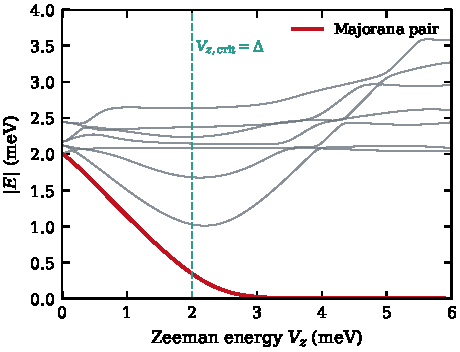
\includegraphics[width=\columnwidth]{fig1_spectrum.pdf}
\caption{BdG excitation spectrum of an $N=80$ chain versus Zeeman energy at
$\mu=0$, $t=20$~meV, $\alpha=10$~meV, $\Delta=2$~meV. The bulk gap closes at
$\vzc=\Delta=2$~meV (green dashed) and a Majorana pair (red) pins to zero
energy in the topological phase. Grey: bulk states.}
\label{fig:spectrum}
\end{figure}

% =====================================================================
\section{The operational gap and its optimum}
\label{sec:optimum}

The quantity that governs protection is not $\vzc$ but $\dtop$, the lowest
bulk excitation at the operating point. Two minima of Eq.~(\ref{eq:hk})
compete for it:
%
\begin{align}
\text{$k=0$ branch:}\quad & \left|\vz - \sqrt{\mu^2+\Delta^2}\right|,
  \quad \text{rising in } \vz, \label{eq:branch0}\\
\text{finite-$k$ branch:}\quad & \approx 0.97\,\Delta \ \ \text{at } ka\approx0.94,
  \quad \text{$\vz$-independent.} \label{eq:branchk}
\end{align}
%
The operational gap is the smaller of the two. Equation~(\ref{eq:branch0})
grows without bound as $\vz$ increases, but Eq.~(\ref{eq:branchk}) caps it,
giving the central result
%
\begin{equation}
\boxed{\ \dtop \le \Delta, \quad \text{approached at } \vz \approx 2\Delta.\ }
\label{eq:bound}
\end{equation}
%
Figure~\ref{fig:branches} shows the crossover explicitly. The two dashed
curves are Eqs.~(\ref{eq:branch0}) and (\ref{eq:branchk}); the solid curve is
the exact gap.

\begin{figure}[t]
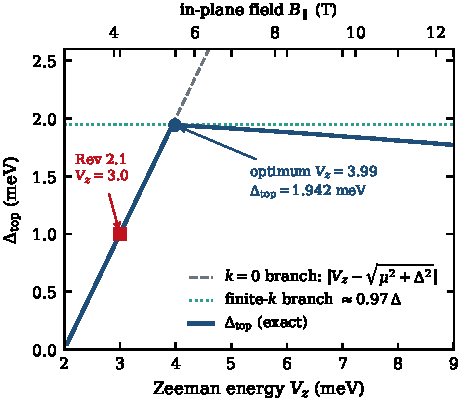
\includegraphics[width=\columnwidth]{fig2_branches.pdf}
\caption{Operational gap versus Zeeman energy at $\mu=0$, $\Delta=2$~meV. The
$k=0$ branch (grey dashed) rises without bound; the finite-$k$ branch (green
dotted) caps it near $0.97\Delta$. The exact gap (blue) is the smaller of the
two, peaking at $\vz=3.95$~meV with $\dtop=1.944$~meV. The choice
$\vz=3$~meV (red square) sits on the rising branch and yields only
$\dtop=1.000$~meV. Upper axis: in-plane field at $g=25$.}
\label{fig:branches}
\end{figure}

The practical consequence is immediate. A specification that chooses
$\vz = 1.5\Delta$ sits on the $k=0$ branch and obtains $\dtop = \Delta/2$;
moving to $\vz \approx 2\Delta$ obtains $\dtop \approx \Delta$. At
$\Delta = 2$~meV this is the difference between $1.000$~meV and $1.944$~meV,
with no change to any material parameter. Table~\ref{tab:compare} collects the
downstream consequences.

\begin{table}[t]
\caption{Operating point at $\Delta = 2$~meV, $\mu = 0$. Both columns are
computed with the same model; the left column is the previously specified
choice $\vz = 1.5\Delta$.}
\label{tab:compare}
\begin{ruledtabular}
\begin{tabular}{lcc}
Quantity & $\vz = 3.00$~meV & $\vz = 3.95$~meV \\
\hline
In-plane field $B_\parallel$ & 4.15 T & 5.46 T \\
$\dtop$ & 1.000 meV & \textbf{1.944 meV} \\
$\dtop/\kB T$ at 0.3 K & 38.7 & \textbf{75.4} \\
$T_{\max} = \dtop/20\kB$ & 0.58 K & \textbf{1.13 K} \\
$e^{-\dtop/\kB T}$ at 0.3 K & $1.6\times10^{-17}$ & $1.8\times10^{-33}$ \\
$\xi$ & 19.1 sites & \textbf{10.8 sites} \\
$L = 30\xi$ & 5.73 $\mu$m & \textbf{3.24 $\mu$m} \\
$\hbar/\dtop$ & 0.66 ps & 0.34 ps \\
Field alignment & $0.0276^\circ$ & $0.0210^\circ$ \\
\end{tabular}
\end{ruledtabular}
\end{table}

The approach to the bound in Eq.~(\ref{eq:bound}) is not exact and tightens as
$\Delta$ decreases: we find $\dtop/\Delta = 0.999,\ 0.992,\ 0.972,\ 0.943$ at
$\Delta = 0.5,\ 1.0,\ 2.0,\ 3.0$~meV respectively. The bound is therefore
sharpest precisely where the architecture is closest to failing, which is the
regime that matters.

\subsection{Localisation length and channel length}

Because $\xi$ scales inversely with the gap, optimising $\vz$ also shortens the
Majorana localisation length, from $19.1$ to $10.8$ sites
(Fig.~\ref{fig:localisation}). Requiring $L \ge 30\xi$ to suppress end-mode
hybridisation below $0.1$~feV, the production channel shortens from
$5.73$~$\mu$m to $3.24$~$\mu$m. For a per-flake exfoliation process in which
die area is the yield driver, this is a material secondary benefit.

\begin{figure}[t]
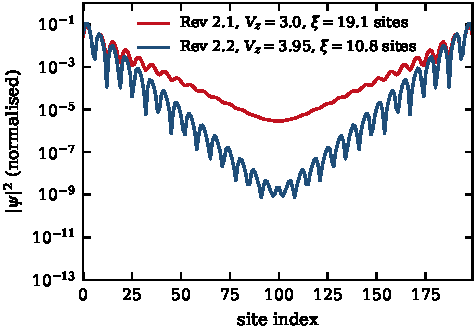
\includegraphics[width=\columnwidth]{fig5_localisation.pdf}
\caption{Site-resolved Majorana probability density at $N=200$ for the two
operating points. Optimising $\vz$ shortens $\xi$ from $19.1$ to $10.8$ sites,
because $\xi \propto 1/\dtop$.}
\label{fig:localisation}
\end{figure}

% =====================================================================
\section{The accessible operating region}
\label{sec:map}

The Zeeman energy is set by the in-plane field,
$\vz = \tfrac{1}{2}g\mu_{\rm B}B_\parallel$, so with $g\approx25$ a $16$~T
magnet caps $\vz$ at $11.6$~meV. This constraint binds the optimisation and
must be imposed: because the $k=0$ expression Eq.~(\ref{eq:branch0}) grows
monotonically, an unconstrained search that evaluates only the closed form will
report the edge of its own scan range as an optimum. Figure~\ref{fig:map} shows
$\dtop$ over the $(\mu,\vz)$ plane with the optimum locus and two magnet
ceilings overlaid.

\begin{figure}[t]
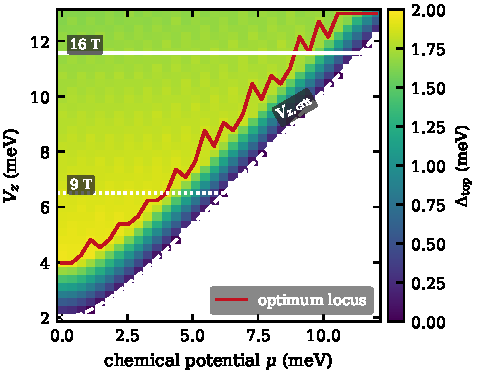
\includegraphics[width=\columnwidth]{fig3_map.pdf}
\caption{$\dtop$ over the $(\mu,\vz)$ plane at $\Delta = 2$~meV. White dashed:
the phase boundary $\vzc=\sqrt{\mu^2+\Delta^2}$. Red: the optimum locus,
tracking $\vz\approx 2\vzc$. White horizontal lines: $9$~T and $16$~T ceilings
at $g=25$. Beyond $\mu\approx10$~meV the optimum is no longer reachable at
$16$~T.}
\label{fig:map}
\end{figure}

The chemical potential is free over a useful range. Between $\mu = 0$ and
$\mu = 8$~meV the optimised gap falls only from $1.944$ to $1.792$~meV, a
degradation of $8\%$, provided the field is available to reach
$\vz \approx 2\sqrt{\mu^2+\Delta^2}$. Beyond $\mu\approx 10$~meV the $16$~T
ceiling binds and $\dtop$ drops sharply.

This reframes a constraint usually quoted as a materials requirement. The
condition $E_F \lesssim 8$~meV is often inherited from the vortex-core
mini-gap argument, which does not apply to a gate-defined channel. What
actually limits $\mu$ here is magnet access: at $16$~T, $\mu \le 8$~meV; at
$9$~T, $\mu \lesssim 4$~meV. The distinction matters because the reported
suppression mechanisms for cuprate-to-TI proximity include a small
topological-surface-state Fermi surface~\cite{Wang2014}; if that effect is
significant, operating at $\mu = 4$--$8$~meV is available at a cost of
$\le 8\%$ in $\dtop$.

% =====================================================================
\section{Comparison with the vortex-core route}
\label{sec:comparison}

Margalit \emph{et al.}~\cite{Margalit2022} proximitise a large-Rashba
substrate with a twisted cuprate bilayer under an out-of-plane field, binding
MZMs in vortex cores. Their topological gap descends from the induced pairing
through an explicit reduction chain,
%
\begin{equation}
\delta E = \Delta \times \tfrac{1}{2} \times (\alpha/t)^2 \times (a_0/a)^2 ,
\label{eq:chain}
\end{equation}
%
with $\alpha = 76$~meV, $t = 132$~meV and five unit cells per moir\'e
supercell, giving a total factor of approximately $1/30$. From their stated
reasonable estimate $\kappa\Delta_{\rm SC}\approx 1$~meV for the induced
pairing, Eq.~(\ref{eq:chain}) yields $\delta E \approx 0.033$~meV.

Both suppressions are structural to that mechanism: the $(\alpha/t)^2$ arises
because the Chern gap opens at second order in the spin--orbit scale, and the
$(a_0/a)^2$ is moir\'e dilution. The Zeeman-driven channel pays neither. Its
gap is first order in the pairing, Eq.~(\ref{eq:bound}), because it is not a
second-order Chern gap and there is no moir\'e cell. Applying the criterion
$\dtop/\kB T \ge 20$ to both:

\begin{table}[h]
\caption{Mechanism comparison. These are different physical systems; the
comparison is of mechanisms, not a like-for-like device benchmark. Both
numbers are model calculations and neither is measured.}
\label{tab:mechanism}
\begin{ruledtabular}
\begin{tabular}{lcc}
Route & topological gap & $T_{\max}$ \\
\hline
Vortex / Chern~\cite{Margalit2022} & 0.033 meV & 19 mK \\
Gate-defined Zeeman channel & 1.944 meV & \textbf{1.13 K} \\
\end{tabular}
\end{ruledtabular}
\end{table}

The ratio is roughly a factor of $60$ in operating temperature, and it is the
difference between requiring a dilution refrigerator and not. It follows from
the published reduction chain rather than from any disagreement with it.

Two secondary points. Reference~\cite{Margalit2022} uses Bi-2201 (single
CuO$_2$ layer, bulk pairing $\sim12$~meV) whereas this architecture assumes
Bi-2212 ($\sim40$~meV), so roughly three times more intrinsic pairing is
available to donate. Separately, vortex-bound MZMs are separated from
Caroli--de Gennes--Matricon levels by a mini-gap
$\delta \simeq \dtop^2/E_F$; at $E_F = 50$--$100$~meV and $\dtop\approx1$~meV
this is $11$--$22$~$\mu$eV, or $0.4$--$0.9\,\kB T$ at $0.3$~K. For the
proposal of Ref.~\cite{Margalit2022} this is not the binding constraint, since
$\delta E = 0.033$~meV already implies sub-$20$~mK operation; we note it only
as a consideration for vortex-core routes generally.

% =====================================================================
\section{Beyond mean field, and disorder}
\label{sec:dmrg}

BdG is a mean-field description. To test whether the topological phase
survives interactions we map the spinless effective model
(Zeeman-polarised band) to a spin chain by Jordan--Wigner transformation,
%
\begin{align}
H =\ & -\tfrac{\mu}{2}\sum_j Z_j
      - \tfrac{t-\Delta}{2}\sum_j X_j X_{j+1}
      - \tfrac{t+\Delta}{2}\sum_j Y_j Y_{j+1} \nonumber\\
     & + \tfrac{V}{4}\sum_j Z_j Z_{j+1},
\end{align}
%
and solve by density-matrix renormalisation group. The order parameter is the
long-distance correlator $\langle Y_i Y_j\rangle$, nonzero exactly in the
topological phase. At $V=0$ the method reproduces the analytic boundary
$\mu_c = 2t$, and ground-state energies agree with exact diagonalisation at
$L=12$ to $2\times10^{-11}$ including with interactions on.

We find that nearest-neighbour Coulomb repulsion does not destroy the phase;
it \emph{widens} the $\mu$-window, with $\mu_c$ moving from $2.0$ to $3.0$ in
units of $t$ at $V = t$. Going beyond mean field therefore makes the
gate-voltage window more forgiving rather than less, consistent with prior
work on interacting Majorana wires~\cite{Stoudenmire2011}.

For electrostatic disorder we performed $2204$ DMRG solves ($L = 40, 60, 80,
120$; box disorder $W \le 10$; $50$ realisations per point) with finite-size
scaling. Quoting a tolerance as a fraction of $t$ does not transfer between
models, since the toy chain runs at gap/$t\sim1$ while the device runs at
$\sim0.05$; the transferable quantity is $\delta\mu_{\rm rms}/\dtop$, with
$\delta\mu_{\rm rms} = W/\sqrt{12}$. At the criterion corresponding to onset of
degradation we obtain
%
\begin{equation}
\delta\mu_{\rm rms}/\dtop \approx 0.9 \pm 0.15 .
\end{equation}
%
We report this as a bound rather than a converged value: all four collapse
criteria are non-monotonic in $1/L$ at $50$ realisations, indicating that
sampling noise exceeds the finite-size trend. A separate convergence run at
larger bond dimension revealed Griffiths-like multistability---paired runs on
identical disorder realisations converging to distinct minima with energy
differences of order $10^{-3}t$---which we address by multi-restart
optimisation. The engineering conclusion (the phase tolerates disorder well in
excess of realistic gated-TI potential variance) is robust; the precise
threshold is not.

% =====================================================================
\section{The decisive measurement}
\label{sec:milestone}

Every result above is conditional on $\Delta$, the proximity-induced pairing
gap in the Bi$_2$Se$_3$ surface beneath a cold-stacked $45^\circ$ bilayer.
This quantity cannot be computed: cuprate superconductivity has no accepted
microscopic theory, so the pairing in the parent material---and hence what it
induces across an interface---is not obtainable from first principles.
Theoretical estimates treat it as an input.

The experiment is tunneling spectroscopy (STM or planar junction) into the
proximitised TI surface at zero field, with no gating, channel definition or
device fabrication. Because tunneling resolution is $\approx 3.5\kB T$, a
$2$~meV gap is comfortably resolved at $1$~K ($3.5\kB T = 0.30$~meV) and
marginally at $4.2$~K; a dilution refrigerator is not required.
Figure~\ref{fig:tunneling} gives predicted spectra.

\begin{figure}[t]
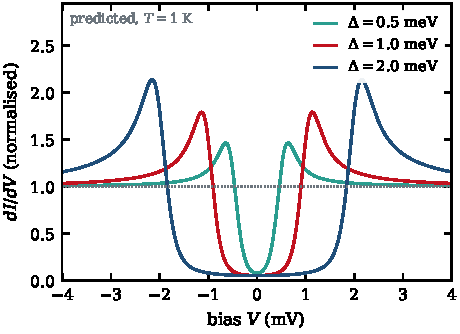
\includegraphics[width=\columnwidth]{fig6_tunneling.pdf}
\caption{Predicted tunneling conductance at $T=1$~K for three values of the
induced gap, Dynes-broadened with $\Gamma = 0.05\Delta$. The observable is a
hard gap: zero-bias conductance suppressed to a few percent of normal. A soft
gap ($\gtrsim 0.3$ of normal) would itself be informative.}
\label{fig:tunneling}
\end{figure}

\begin{table}[t]
\caption{Decision thresholds, with $\vz$ re-optimised at each $\Delta$ subject
to a $16$~T ceiling.}
\label{tab:decision}
\begin{ruledtabular}
\begin{tabular}{lccc}
Measured $\Delta$ & $\dtop$ & $T_{\max}$ & Verdict \\
\hline
$<0.50$ meV & $<0.52$ & $<0.30$ K & fails \\
0.50 meV & 0.520 & 0.30 K & marginal \\
1.00 meV & 1.002 & 0.58 K & viable \\
2.00 meV & 1.944 & 1.13 K & design point \\
3.00 meV & 2.825 & 1.64 K & comfortable \\
\end{tabular}
\end{ruledtabular}
\end{table}

Figure~\ref{fig:robustness} shows why the re-optimisation matters for
robustness. With $\vz$ held fixed, $\dtop$ is a non-monotonic function of
$\Delta$, peaking near $\Delta \approx 1.5$~meV and falling thereafter---an
artifact of the fixed operating point, not a property of the model. With $\vz$
re-optimised the dependence is monotonic, and the architecture tolerates half
the induced pairing for the same performance. In particular
$\Delta = 1$~meV---the reasonable estimate of Ref.~\cite{Margalit2022}---moves
from marginal ($0.29$~K) to comfortable ($0.58$~K).

\begin{figure}[t]
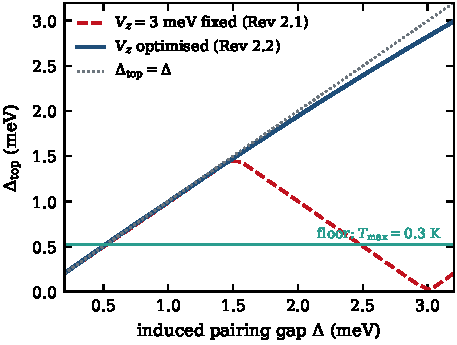
\includegraphics[width=\columnwidth]{fig4_robustness.pdf}
\caption{$\dtop$ versus induced pairing. Red dashed: $\vz$ fixed at $3$~meV,
showing spurious non-monotonicity. Blue: $\vz$ re-optimised at each $\Delta$,
monotonic and approaching the bound $\dtop = \Delta$ (grey dotted). Green: the
$T_{\max}=0.3$~K floor.}
\label{fig:robustness}
\end{figure}

\emph{Experimental context.} Proximity from a cuprate into a TI is contested.
Angle-resolved photoemission on Bi$_2$Se$_3$ grown \emph{in situ} on Bi-2212
found no induced gap down to $1.5$ quintuple layers~\cite{Wang2014}, attributed
to the short $c$-axis coherence length, incompatible crystal and pairing
symmetries, a small surface-state Fermi surface, and strong spin--orbit
coupling. A scanning-tunneling study subsequently attributed an apparent gap in
the same system to Coulomb blockade rather than superconductivity. Conversely,
proximity-induced superconductivity persisting to at least $80$~K has been
reported in Bi$_2$Se$_3$ and Bi$_2$Te$_3$ bonded mechanically to
Bi-2212~\cite{Wang2012}. The pattern across these results is that growth-based
interfaces fail while mechanically bonded ones succeed, consistent with the
sub-unit-cell $c$-axis coherence length requiring an atomically clean,
adsorbate-free interface. Crucially, the symmetry objection of
Ref.~\cite{Wang2014} applies to a single $d$-wave layer; the $45^\circ$ twist
converts the pairing to fully gapped $d+id'$, which is the configuration that
has not been tested. A positive result must exclude Coulomb blockade.

% =====================================================================
\section{Limitations}
\label{sec:limitations}

\begin{enumerate}
\item \textbf{The induced gap is unmeasured} and every protection budget scales
exponentially with it. This is the load-bearing assumption.
\item \textbf{Not room temperature.} At $300$~K the criterion demands
$\dtop \approx 517$~meV, a bare pairing of order $1$~eV. No thermal engineering
alters $\kB T$.
\item \textbf{The field requirement increases.} Optimisation raises
$B_\parallel$ from $4.15$ to $5.46$~T and correspondingly tightens the
alignment tolerance to $0.0210^\circ$, since the out-of-plane bound
$B_\perp \le 2$~mT that excludes pancake vortices is unchanged.
\item \textbf{Per-flake assembly.} Cold-stacked, angle-locked, adsorbate-free
junctions remain low-throughput.
\item \textbf{The disorder threshold is a bound}, not a converged value.
\item \textbf{The platform is not novel to this work.} Twisted-cuprate MZM
proposals are established~\cite{Margalit2022,Zhu2023}; the contribution here is
the operating-point analysis, the gate-defined channel variant, and the
budgets.
\end{enumerate}

% =====================================================================
\section{Conclusion}

The operational gap of a Zeeman-driven gate-defined Majorana channel is bounded
by the induced pairing gap, $\dtop \le \Delta$, and nearly saturates that bound
at $\vz \approx 2\Delta$. Adopting this operating point rather than
$\vz = 1.5\Delta$ nearly doubles $\dtop$ at fixed materials, raising
$T_{\max}$ from $0.58$ to $1.13$~K and halving the required channel length,
at a cost of $1.3$~T in applied field and a tightened alignment tolerance. The
chemical potential is free over $0 \le \mu \lesssim 8$~meV subject to magnet
access, which reframes the commonly quoted $E_F \lesssim 8$~meV condition.

Whether any of this is realisable rests on a single measurement---the induced
gap under a cold-stacked $45^\circ$ twist junction---which requires $1$~K
rather than dilution temperatures and no device fabrication. The optimisation
reported here lowers the bar that measurement must clear: an induced gap of
$1$~meV, at the low end of published estimates, now suffices.

\begin{acknowledgments}
Numerical work used the open-source \texttt{topological-vqpu} stack; all
figures are reproducible from it.
\end{acknowledgments}

% =====================================================================
\begin{thebibliography}{99}

\bibitem{Kitaev2001} A.~Y. Kitaev, Phys.-Usp. \textbf{44}, 131 (2001).
\bibitem{Nayak2008} C. Nayak, S.~H. Simon, A. Stern, M. Freedman, and
  S. Das Sarma, Rev. Mod. Phys. \textbf{80}, 1083 (2008).
\bibitem{Lutchyn2010} R.~M. Lutchyn, J.~D. Sau, and S. Das Sarma,
  Phys. Rev. Lett. \textbf{105}, 077001 (2010).
\bibitem{Oreg2010} Y. Oreg, G. Refael, and F. von Oppen,
  Phys. Rev. Lett. \textbf{105}, 177002 (2010).
\bibitem{FuKane2008} L. Fu and C.~L. Kane, Phys. Rev. Lett. \textbf{100},
  096407 (2008).
\bibitem{Can2021} O. Can \emph{et al.}, Nat. Phys. \textbf{17}, 519 (2021).
\bibitem{Zhao2023} S.~Y.~F. Zhao \emph{et al.}, Science \textbf{382}, 1422
  (2023).
\bibitem{Margalit2022} G. Margalit, B. Yan, M. Franz, and Y. Oreg,
  Phys. Rev. B \textbf{106}, 205424 (2022), arXiv:2209.11080.
\bibitem{Zhu2023} High-temperature Majorana corner modes in a $d+id'$
  superconductor heterostructure, Phys. Rev. B \textbf{107}, 235125 (2023),
  arXiv:2306.07468.
\bibitem{Karzig2017} T. Karzig \emph{et al.}, Phys. Rev. B \textbf{95},
  235305 (2017).
\bibitem{Stoudenmire2011} E.~M. Stoudenmire, J. Alicea, O.~A. Starykh, and
  M.~P.~A. Fisher, Phys. Rev. B \textbf{84}, 014503 (2011).
\bibitem{Wang2014} E. Wang \emph{et al.}, Absence of a proximity effect in a
  topological insulator on a cuprate superconductor, arXiv:1403.4184.
\bibitem{Wang2012} P. Wang \emph{et al.}, Proximity-induced high-temperature
  superconductivity in the topological insulators Bi$_2$Se$_3$ and
  Bi$_2$Te$_3$, Nat. Commun. \textbf{3}, 1056 (2012).

\end{thebibliography}

\end{document}
